%% IEEE T-BIOM submission -- DISCERN journal extension
%% Template: IEEEtran (tbiom/docs/IEEE_TBIOM/IEEEtran)
%% Every numeric value in the tables is generated by analysis/tbiom/paper/build_tables.py
%% from the committed reports in tbiom/reports/. Do not edit tables/*.tex by hand.
\documentclass[journal]{IEEEtran}

\usepackage{amsmath,amssymb,amsfonts}
\usepackage{booktabs}
\usepackage{graphicx}
\usepackage{url}
\usepackage{multirow}
\usepackage[hidelinks]{hyperref}
\usepackage{tikz}
\usetikzlibrary{arrows.meta,positioning,fit,backgrounds}

\newcommand{\app}{\ensuremath{A}}
\newcommand{\om}{\ensuremath{O}}
\newcommand{\tmp}{\ensuremath{T}}
\newcommand{\pcrp}{PCR6\textsuperscript{+}}

\begin{document}

\title{Complementary Spatial and Temporal Evidence for\\ Reliable Deepfake Video Detection}

\author{Muhammad~Umar~Farooq,~Kutub~Uddin,~Awais~Khan,~and~Khalid~Malik%
\thanks{The authors are with the College of Innovation and Technology, University of Michigan, Flint, MI 48502 USA
(e-mail: \{mufarooq, kutub, mawais, drmalik\}@umich.edu).}%
\thanks{This work extends our conference paper~\cite{discern}, ``Uncertainty-Aware Deepfake Detection via
Multi-View Structural Learning''.}}

\markboth{IEEE Transactions on Biometrics, Behavior, and Identity Science}%
{Author \MakeLowercase{\textit{et al.}}: Complementary Spatial and Temporal Evidence for Reliable Deepfake Video Detection}

\maketitle

\begin{abstract}
Deepfake detectors that read a single face crop have become very strong on face swapping, where the manipulation leaves a per-frame trace. They remain weak on face reenactment, where the frames can be individually plausible and the manipulation lives in how the face moves. We study this asymmetry directly and address it with an evidential formulation in which appearance, off-manifold and temporal evidence are combined as subjective opinions rather than averaged logits. Each view emits a Dirichlet opinion; per-view reliability enters as evidence scaling fitted on source-grouped development folds; and the opinions are combined with the direct multi-source \pcrp{} rule, which -- unlike Dempster's rule and unlike plain PCR6 -- guarantees that a view the reliability fit has discounted to zero behaves exactly as a removed view. Holding the spatial evidence fixed at a strong baseline's own values and adding only the temporal view, the system is ahead of that baseline on $39$ of the $41$ generator--source entries of DF40. The margin is small on face swapping, where both systems exceed $0.97$ AUROC, and large on reenactment ($+0.164$ mean), including four generators on which both spatial views sit at chance and the temporal view alone reaches $0.94$--$0.99$. Across ten cross-dataset benchmarks the system attains a mean video AUROC of $0.9129$, the best of the ten systems compared. A family-resolved ablation shows the three views dividing the work rather than duplicating it: the temporal view carries reenactment, the off-manifold view contributes on every evaluation group, and the appearance view earns its place on swap and in-the-wild content.
\end{abstract}

\begin{IEEEkeywords}
Deepfake detection, face reenactment, evidential deep learning, subjective logic, information fusion, conflict redistribution, uncertainty quantification, video forensics.
\end{IEEEkeywords}

\section{Introduction}
\IEEEPARstart{F}{ace} manipulation methods have separated into two families that make very different demands on a detector. \emph{Face swapping} transplants an identity into a target video and, in doing so, leaves per-frame evidence: blending seams, colour and resolution mismatch, warping near the mask boundary. \emph{Face reenactment} instead drives a target face with a source performance. The identity is untouched, each frame can be a photometrically clean rendering of a real person, and what is wrong is the motion -- expression dynamics, head-pose coupling, the timing of blinks and mouth closure.

Most recent detectors are trained and evaluated in a way that rewards the first family. They consume one aligned crop, they are scored on datasets dominated by swaps, and they have become very accurate there. Our own conference system~\cite{discern} is no exception. The consequence is visible when a detector meets a reenactment generator that renders cleanly: the per-frame evidence simply is not present, and a spatial detector has nothing to read.

This paper starts from that asymmetry and treats it as an evidence problem rather than an architecture problem. We keep the spatial evidence of a strong baseline \emph{fixed}, add a temporal view that sees motion, and ask how the three bodies of evidence should be combined when they are of unequal and input-dependent reliability, and when they sometimes flatly disagree.

Three design commitments follow. First, each view emits a \emph{subjective opinion} -- a Dirichlet over the binary frame with an explicit vacuity mass -- rather than a logit, so that ``this view has little to say here'' is representable and is not confused with ``this view says the two classes are equally likely''. Second, per-view reliability is fitted on source-grouped development folds and applied as \emph{evidence scaling}, which is the discount our system implements and which differs from classical belief-mass discounting everywhere except at its endpoints. Third, the opinions are combined with the direct multi-source \pcrp{} rule of Dezert \emph{et al.}~\cite{pcr6plus}. That last choice is not cosmetic. The reliability fit routinely drives a view's weight to zero, and a zero-weighted view is exactly the vacuous source whose neutrality Dempster's rule and plain PCR6 both violate: under \pcrp{} removing such a view changes the fused opinion by exactly zero, whereas under PCR6 it can change it by up to $0.28$.

Our contributions are:

\begin{enumerate}
\item \textbf{A controlled demonstration of spatial--temporal complementarity.} Holding two spatial views frozen at a strong baseline's own values and adding only an adapted V-JEPA\,2 temporal view, the system is ahead on $39$ of $41$ DF40 generator--source entries. The gain is concentrated exactly where the mechanism predicts: $+0.164$ mean AUROC on reenactment against $+0.009$ on swapping (Sec.~\ref{sec:df40}).
\item \textbf{An evidential fusion formulation whose operator respects the reliability it is given.} We specify the opinion construction, the evidence-scaling discount and direct multi-source \pcrp{} fusion, and we verify the vacuous-view neutrality property algebraically on the implemented binary domain (Sec.~\ref{sec:fusion}, Table~\ref{tab:operators}).
\item \textbf{A family-resolved account of what each view contributes.} Removing the temporal view costs $0.151$ AUROC on DF40 reenactment; removing the off-manifold view costs on every evaluation group; removing the appearance view costs on swap and in-the-wild content while helping slightly on reenactment. The three views divide the work by manipulation family rather than duplicating it, and the fitted reliability is what lets each step aside where it is uninformative (Sec.~\ref{sec:views}).
\item \textbf{A reliability and robustness account} covering calibration, error ranking by fused vacuity, selective prediction, and evaluation-time JPEG and resize corruption (Sec.~\ref{sec:reliability}).
\end{enumerate}

\section{Related Work}

\subsection{Generalising deepfake detectors}
Cross-dataset generalisation has been pursued through blending-artifact simulation, frequency cues, and large pretrained visual backbones adapted with lightweight modules. Recent strong baselines in our comparison -- GenD variants, Effort, ForAda, FSFM~\cite{gend,effort,forada,fsfm} -- differ mainly in which pretrained representation they adapt and how they regularise it. They are spatial: each consumes an aligned face crop. Our results show these systems clustering tightly on swap-dominated benchmarks and separating sharply on reenactment, which is the behaviour this paper sets out to explain and correct.

\subsection{Temporal modelling for face forgery}
Temporal approaches range from optical-flow and landmark-dynamics features to video transformers. Self-supervised video representations such as V-JEPA\,2~\cite{vjepa2} are attractive here because they are trained to predict in representation space and therefore encode motion regularities without requiring forgery labels. We adapt such a backbone with low-rank adapters rather than full fine-tuning, which keeps the temporal view a bounded addition to an existing spatial system.

\subsection{Evidential learning and multi-view fusion}
Evidential deep learning~\cite{edl} places a Dirichlet over the class simplex so that a prediction carries an explicit vacuity. In multi-view settings the question becomes how to combine opinions. Trusted multi-view classification uses Dempster's rule; RCML~\cite{rcml} argues that Dempster's rule understates uncertainty under conflict and instead aggregates opinions by averaging, proving that fused uncertainty then increases for conflictive instances; Discounted Belief Fusion~\cite{dbf} measures a pairwise degree of conflict and converts it into per-modality discounts before an order-invariant fusion. Our setting differs in that reliability is fitted once on development folds rather than inferred per sample, and the operator is chosen for a property -- neutrality of a discounted-away view -- that matters precisely because fitted reliabilities reach zero.

\subsection{Conflict redistribution}
Dempster's rule normalises conflicting mass away, which is what produces its well-known counter-intuitive behaviour under strong disagreement. Proportional conflict redistribution rules instead return conflicting mass to the sources that produced it~\cite{pcr}. PCR6 is the standard multi-source form; Dezert \emph{et al.}~\cite{pcr6plus} show that PCR5 and PCR6 can still assign conflicting mass to an ignorant source, and restore neutrality of the vacuous belief assignment through binary keeping indexes, giving PCR5\textsuperscript{+} and \pcrp{}. We use the direct multi-source \pcrp{} rule and credit it as theirs; our contribution here is its application to a reliability-discounted three-view detector and the demonstration that the property it restores is one our system actually exercises.

\subsection{Relation to the conference version}
This paper extends~\cite{discern}, which combined visual, semantic-predicate and structural streams under a
Dirichlet evidential framework with confidence-modulated fusion, inter-branch disagreement calibration and
per-stream auxiliary supervision, evaluated on five cross-dataset benchmarks. Table~\ref{tab:extension} states what
is retained, modified, replaced, removed and new. In short: the evidential treatment of heterogeneous streams is
retained; the semantic-predicate stream is removed and the structural stream replaced by a single off-manifold
deviation score; a temporal view is added; the two fusion mechanisms are replaced by a fitted reliability discount and
a conflict-redistribution rule; and the evaluation is extended from five benchmarks to ten plus $41$ DF40
generator--source entries. The reenactment failure this paper addresses is not visible at five swap-dominated
benchmarks, which is why it was not identified in the conference version.

% HAND-WRITTEN, not generated by build_tables.py (qualitative content).
% Sources: DISCERN paper (tbiom/docs/DISCERN.pdf, Secs. 1, 3.3, 3.4) and this system's configs
% (DISCERN_Ext warm_dicome_gate_seed42.yaml, analysis/tbiom/temporal/train_branch.py).
\begin{table*}[t]
\centering
\caption{Relation to the conference version~\cite{farooq2026discern}. The extension keeps the evidential treatment of
heterogeneous streams and replaces everything about how those streams are constituted and combined.}
\label{tab:extension}
\small
\begin{tabular}{p{0.20\textwidth}p{0.10\textwidth}p{0.30\textwidth}p{0.30\textwidth}}
\toprule
Conference component & Status & This paper & Why \\
\midrule
Visual stream: CLIP with layer-norm tuning & modified & appearance view \app{}: CLIP ViT-L with LoRA adapters on the attention projections & adapters leave the backbone untouched, so the view can be frozen and reused as a fixed body of evidence \\
Semantic stream: differentiable predicates over facial signals (expression--action-unit alignment, pose--gaze consistency, geometric symmetry) & removed & --- & the predicates are per-frame and appearance-derived; they do not address the reenactment failure this paper targets \\
Structural stream: class-dependent dependency modelling, retained as interpretable structure & replaced & off-manifold view \om{}: a $\beta$-VAE head on the same CLIP path, scoring distance from the genuine-face manifold & a single scalar deviation score proved to be the more reliable of the two spatial signals, contributing on every evaluation group (Table~\ref{tab:viewrole}) \\
--- & new & temporal view \tmp{}: V-JEPA\,2 ViT-L with LoRA adapters and an evidential head on ordered clips & the conference system had no access to motion, which is the only channel in which a cleanly rendered reenactment differs from a real video \\
Confidence-modulated evidence fusion & replaced & reliability as evidence scaling, $e'=r\,e$, fitted per fold on source-grouped development folds & a fitted per-view reliability is auditable and can be reported per fold; it also makes zero weights explicit rather than implicit \\
Inter-branch disagreement calibration & replaced & direct multi-source \pcrp{} with retained conflict mass $K$ & conflict is redistributed to the views that produced it and reported, instead of being converted into a calibration penalty during training \\
Per-stream auxiliary supervision & retained & per-view evidential supervision in the spatial checkpoint & unchanged from the conference recipe \\
Evaluation: five cross-dataset benchmarks & extended & ten cross-dataset benchmarks, $41$ DF40 generator--source entries, and two evaluation-time processing conditions & the swap/reenactment asymmetry is invisible at five swap-dominated benchmarks \\
\bottomrule
\end{tabular}
\end{table*}


\section{Method}
\label{sec:method}

\subsection{Overview}
The system scores a video with three evidential views (Fig.~\ref{fig:arch}). Two are spatial and operate on aligned face crops: an \emph{appearance} view \app{} and an \emph{off-manifold} view \om{}. One is temporal: an adapted video encoder \tmp{} that consumes an ordered clip. Each view emits a binary Dirichlet opinion per frame or clip. Opinions are averaged per video, discounted by a per-view reliability fitted on development folds, and combined with direct multi-source \pcrp{}. The fused opinion yields a probability, a vacuity, and a retained conflict mass.

\begin{figure}[t]
\centering
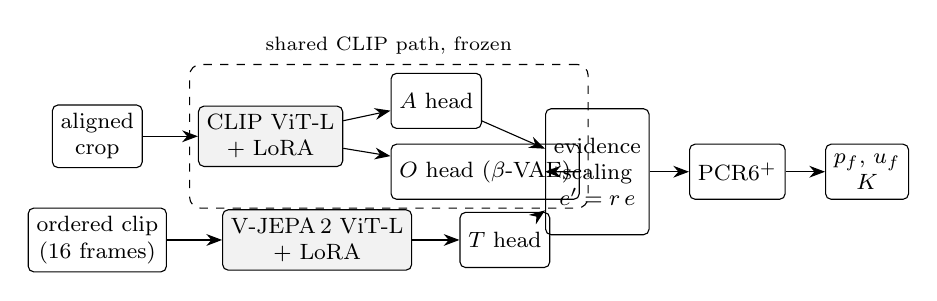
\begin{tikzpicture}[
  font=\footnotesize,
  box/.style={draw,rounded corners=2pt,align=center,inner sep=3pt,minimum height=7mm},
  ev/.style={box,fill=black!5},
  >={Stealth[length=2mm]}]
\node[box] (crop) {aligned\\crop};
\node[box,below=5mm of crop] (clip) {ordered clip\\(16 frames)};
\node[ev,right=7mm of crop] (clip4) {CLIP ViT-L\\+ LoRA};
\node[ev,right=7mm of clip] (vj) {V-JEPA\,2 ViT-L\\+ LoRA};
\node[box,right=6mm of clip4,yshift=4.5mm] (a) {\app{} head};
\node[box,right=6mm of clip4,yshift=-4.5mm] (o) {\om{} head ($\beta$-VAE)};
\node[box,right=6mm of vj] (t) {\tmp{} head};
\node[box,right=8mm of a,yshift=-9mm,minimum height=16mm] (disc) {evidence\\scaling\\$e'=r\,e$};
\node[box,right=5mm of disc] (fuse) {\pcrp{}};
\node[box,right=5mm of fuse,align=center] (out) {$p_f$, $u_f$\\$K$};
\draw[->] (crop) -- (clip4);
\draw[->] (clip) -- (vj);
\draw[->] (clip4) -- (a);
\draw[->] (clip4) -- (o);
\draw[->] (vj) -- (t);
\draw[->] (a) -- (disc);
\draw[->] (o) -- (disc);
\draw[->] (t) -- (disc);
\draw[->] (disc) -- (fuse);
\draw[->] (fuse) -- (out);
\begin{scope}[on background layer]
\node[draw,dashed,rounded corners,fit=(clip4)(a)(o),inner sep=3pt,label=above:{\scriptsize shared CLIP path, frozen}] {};
\end{scope}
\end{tikzpicture}
\caption{The three-view evidential system. The appearance and off-manifold heads share one CLIP feature path and are frozen at the baseline's values; only the temporal view is added and adapted. Reliability enters as evidence scaling before fusion.}
\label{fig:arch}
\end{figure}

\subsection{Views}
\label{sec:views-def}

\textbf{Appearance (\app{}).} A CLIP ViT-L/14 encoder adapted with LoRA~\cite{lora} (rank $8$, $\alpha=16$, dropout $0.1$, on the query and value projections), followed by a projection to a $64$-dimensional feature and an evidential head.

\textbf{Off-manifold (\om{}).} A $\beta$-VAE~\cite{betavae} head ($32$-dimensional latent, $\beta_{\mathrm{KLD}}=2.0$) attached to the same CLIP feature path, trained with a reconstruction and KL objective alongside the classification loss. It scores how far a crop lies from the manifold of genuine faces. Because \app{} and \om{} read one feature path, their evidence is not independent -- a fact that matters for both the fusion operator and the ablations.

\textbf{Temporal (\tmp{}).} A V-JEPA\,2 ViT-L encoder consuming $16$ frames sampled uniformly and \emph{in order} over the stored crops of a video. All backbone weights are frozen; LoRA adapters (rank $8$, $\alpha=16$, dropout $0.1$) are inserted in the attention query and value projections of every layer, and an evidential head (LayerNorm $\rightarrow$ $128$ GELU $\rightarrow$ $2$, softplus) is trained on mean-pooled tokens. Training uses FF++ c23 training videos only, class-balanced sampling, AdamW (weight decay $0.01$, cosine schedule to $10^{-6}$, bf16), $10$ epochs, batch $32$, learning rates $2\!\times\!10^{-4}$ for adapters and $2\!\times\!10^{-3}$ for the head, with the evidential loss and annealed KL. A shared-processing augmentation is applied to training clips only, drawn independently of the label: no processing with probability $0.40$, JPEG quality $70/50/30$ with probability $0.10$ each, and down--up resize $0.75/0.50/0.35$ with probability $0.10$ each. The checkpoint is selected by the development objective of Sec.~\ref{sec:protocol}.

\textbf{Why these three.} The views are chosen to read different evidence. The appearance view reads the local
photometric record of a manipulation -- blending seams, colour and resolution mismatch, texture inconsistency -- which
is what a swap leaves behind. The off-manifold view asks a different question of the same features, namely how far the
crop lies from the manifold of genuine faces, which does not require the artifact to be nameable. The temporal view
reads motion, which is the only channel in which a cleanly rendered reenactment can betray itself. Section~\ref{sec:views}
shows that this division of labour is real and that each view carries a family the others do not.

\textbf{What is \emph{not} used.} The spatial checkpoint also contains a fourth evidential head, a face-prior branch
distilled from a face-representation model. We evaluated it as a candidate view under the same operator and fitting
procedure; the reliability fit drove its weight to zero in all five folds, whether it was added to the deployed set or
substituted for the appearance view, so the fused system was numerically unchanged by its presence. It is therefore
excluded and the fusion is fixed at three views. The spatial views themselves are frozen: they are warm-started from our trained baseline and not updated. The system's only new trainable component relative to that baseline is the temporal view.

Freezing the spatial views is a deliberate choice, not a convenience. Retraining the spatial encoder alongside a new
temporal branch would confound two changes, and any gain could then be attributed to either. By holding the spatial
evidence at the baseline's own values we make Sec.~\ref{sec:df40} a controlled contrast in which the only difference
between the two systems is the presence of the temporal view and the rule used to combine the evidence. The cost of
this choice is that the system inherits whatever the baseline's spatial views cannot see; the benefit is that the
attribution of the result is unambiguous.

\subsection{Opinions}
We work on the binary frame $\Theta=\{\textit{fake},\textit{genuine}\}$ with a uniform base rate and $W=2$. A view producing non-negative evidence $e_k$ for class $k$ defines a Dirichlet with $\alpha_k=e_k+1$ and $S=\sum_k \alpha_k$, and the corresponding opinion
\begin{equation}
b_k=\frac{e_k}{S},\qquad u=\frac{W}{S},\qquad p_{\textit{fake}} = b_{\textit{fake}} + \frac{u}{2},
\label{eq:opinion}
\end{equation}
with $b_{\textit{fake}}+b_{\textit{genuine}}+u=1$. The projected probability $p_{\textit{fake}}$ is the Dirichlet mean. A view with no evidence has $u=1$ and is \emph{vacuous}.

\subsection{Reliability as evidence scaling}
\label{sec:discount}
Per-view reliability $r_v\in[0,1]$ is applied in the evidence domain,
\begin{equation}
e'_{v,k} = r_v\, e_{v,k},
\label{eq:discount}
\end{equation}
and the discounted opinion is recovered through~\eqref{eq:opinion}. This is \emph{not} classical belief-mass discounting, $m'(A)=r\,m(A)$ for $A\neq\Theta$ with the remainder to $\Theta$; the two agree only at $r=1$ (the identity) and at $r=0$ (both give the vacuous opinion), and differ at intermediate $r$. We state this explicitly because the distinction is easy to lose and because the $r=0$ endpoint is what makes the operator choice in Sec.~\ref{sec:fusion} consequential.

The weights are fitted by grid search over $r_v\in\{0,0.25,0.5,0.75,1\}$ with $\max_v r_v = 1$, maximising the development objective of Sec.~\ref{sec:protocol} on the fitting fold, separately for every arm and every fold. No weight is ever transferred between arms.

\subsection{Fusion by direct multi-source \pcrp{}}
\label{sec:fusion}
Let $X_j=(X_{j1},\dots,X_{jS})$ range over tuples of focal elements, one per view, with $\pi_j=\prod_i m_i(X_{ji})$ and $\pi_j(\emptyset)$ denoting a tuple whose intersection is empty. The direct multi-source PCR6 rule~\cite{pcr} sets $m(\emptyset)=0$ and, for $A\neq\emptyset$,
\begin{equation}
m_{\mathrm{PCR6}}(A)=m_{\mathrm{Conj}}(A)+\!\!\sum_{j\,:\,A\in X_j,\ \pi_j(\emptyset)}\!\!
\frac{\big(\sum_{i:X_{ji}=A} m_i(X_{ji})\big)\,\pi_j(\emptyset)}
{\sum_{X\in X_j}\sum_{i:X_{ji}=X} m_i(X_{ji})}.
\label{eq:pcr6}
\end{equation}
\pcrp{}~\cite{pcr6plus} modifies~\eqref{eq:pcr6} with binary keeping indexes $\kappa_j(\cdot)$, which discard focal elements that contain every other element implied in that partial conflict:
\begin{equation}
m_{\pcrp{}}(A)=m_{\mathrm{Conj}}(A)+\!\!\sum_{j\,:\,A\in X_j,\ \pi_j(\emptyset)}\!\!
\frac{\kappa_j(A)\big(\sum_{i:X_{ji}=A} m_i\big)\,\pi_j(\emptyset)}
{\sum_{X\in X_j}\kappa_j(X)\sum_{i:X_{ji}=X} m_i}.
\label{eq:pcr6p}
\end{equation}
Equation~\eqref{eq:pcr6p} reduces to~\eqref{eq:pcr6} when every keeping index equals one, and for $S=2$ both coincide with PCR5.

On our binary frame the indexes take a simple form. A conflicting tuple must contain both singletons, so its distinct focal elements are $\{\textit{fake}\}$, $\{\textit{genuine}\}$ and, if any view is partly ignorant, $\Theta$. Neither singleton contains the other, so both keep index $1$; $\Theta$ contains both, so $\kappa_j(\Theta)=0$. \textbf{On this domain \pcrp{} is exactly PCR6 with conflicting mass never redistributed to $\Theta$.} We compute the indexes from their definition rather than assuming this, and verify the consequence: a view discounted to $r=0$ leaves the fused opinion unchanged to $0$ under \pcrp{}, while under PCR6 the same removal moves it by up to $0.28$ (Table~\ref{tab:operators}). Since the fitted reliabilities do reach zero in most folds, this is a property the system exercises rather than a theoretical nicety.

\subsection{Aggregation, outputs and decision}
Per-frame opinions are averaged per video before fusion; the temporal view already emits one opinion per clip. Fusion is applied to the video-level opinions. The system outputs the fused probability $p_f$, the fused vacuity $u_f$, and the conflicting mass $K$ accumulated before redistribution, which we also decompose by the pair of views that produced it. The decision threshold is the equal-error-rate point on the FF++ validation split, computed per arm on its own scores and applied unchanged to every evaluation set. Labels are never an inference input.

\section{Experimental Protocol}
\label{sec:protocol}

\subsection{Training and development data}
All trainable components are trained on FaceForensics++ (c23)~\cite{ffpp} training videos only. Development uses three held-out mixes -- \textsc{VALmix}, \textsc{VALmix-v2} and the FF++ validation split -- combined into a development pool that is used for two purposes and no others: selecting checkpoints and fitting the reliability weights.

The development objective is a macro AUROC over three manipulation-type cells (swap, reenactment, in-the-wild), computed over five source-grouped folds produced by \texttt{GroupShuffleSplit} on the source-video identity with seeds $0$--$4$. Grouping by source keeps every manipulated copy of a source video, and its processed variants, in the same fold. \textbf{These five folds are fitting folds, not detector seeds}; they quantify sampling and weight-fitting variability conditional on the trained encoders, not encoder-training variability.

\subsection{Evaluation suites}
We report two suites. The first is ten cross-dataset benchmarks: CDF-v2 and CDF-v3~\cite{celebdf}, DFD~\cite{dfd},
DFDC~\cite{dfdc}, DFDCP~\cite{dfdcp}, DeepfakeEval-2024~\cite{dfeval24}, FFIW~\cite{ffiw}, KoDF~\cite{kodf},
IDForge~\cite{idforge} and DFDM~\cite{dfdm}. The second is DF40~\cite{df40} cross-manipulation, comprising $41$ generator--source entries: ten face-swap and eleven reenactment generators, each in a Celeb-DF-sourced and a FaceForensics++-sourced version, plus DeepFaceLab. Each entry is scored against the genuine pool DF40 ships for its source, so a generator's AUROC is never computed against another source's real videos. We report a family-balanced mean, which weights each of the four family$\times$source cells equally, and a generator-macro mean, which weights each of the $41$ entries equally; the two differ because the Celeb-DF-sourced cells contain more generators.

Processing robustness is evaluated by applying JPEG quality $40$ and down--up resize $0.60$ to the stored crops at evaluation time. These corruptions never appear in any fitting or selection step.

\subsection{Exposure}
CDF-v2 and DeepfakeEval-2024 informed development through diagnosis, and DF40 informed operator design in preceding studies. We therefore describe both suites as exposed benchmark evaluation rather than untouched confirmation, and we do not claim held-out generalisation from them. What the DF40 comparison does establish is a controlled contrast: both systems see identical videos with identical aggregation, and they differ only in the presence of the temporal view and the fusion rule.

\subsection{Metrics}
All detection numbers are video-level AUROC in $[0,1]$. ECE uses $15$ equal-width bins. Error-detection AUROC ranks the system's own mistakes at the frozen threshold using an uncertainty score, with higher indicating a more suspect sample. AURC and E-AURC follow the standard risk--coverage convention~\cite{aurc}, with E-AURC the excess over the optimal ranking. Paired intervals are computed with a source-grouped bootstrap, $2{,}000$ draws, resampling source groups together with all of their linked manipulated and processed copies; a difference must exceed a materiality floor of $10^{-4}$ AUROC to be treated as non-zero, so that two arms differing only by floating-point noise cannot produce a significant interval.

\subsection{Comparators}
Every comparator in Table~\ref{tab:crossdataset} was reproduced locally and scored on the same videos with the same aggregation; no value is copied from a published table. The DF40 comparison uses our own trained instance of the baseline, replayed through its own fusion.

\section{Results}

\subsection{Cross-dataset generalisation}
Table~\ref{tab:crossdataset} reports the ten benchmarks. The proposed system attains the best mean video AUROC, $0.9129$, and leads on CDF-v3 ($0.9639$), KoDF ($0.9600$) and DeepfakeEval-2024 ($0.7235$). It does not lead everywhere: DFDC, DFDCP and DFD are won by spatial baselines. The pattern is consistent with the paper's thesis rather than incidental to it -- the sets where the system leads are those with substantial reenactment or talking-head content, and the sets where it trails are frame-artifact-dominated benchmarks on which strong spatial detectors are already near their ceiling.

% generated by analysis/tbiom/paper/build_tables.py
% source: EXP_PCR6P_EXPOSED.json (ours), BASELINE_MATRIX.json (comparators)
\begin{table*}[t]
\centering
\caption{Cross-dataset generalisation, video-level AUROC. All systems are evaluated locally on the same videos with the same aggregation; no number is taken from a published table. Our rows are means over the five reliability-fitting folds. Best per column in \textbf{bold}.}
\label{tab:crossdataset}
\setlength{\tabcolsep}{4pt}
\small
\begin{tabular}{lccccccccccc}
\toprule
Method & CDF-v2 & CDF-v3 & DFD & DFDC & DFDCP & DFEval24 & FFIW & KoDF & IDForge & DFDM & Mean \\
\midrule
DISCERN (conf.\ version) & 0.9509 & 0.8954 & \textbf{0.9431} & \textbf{0.8879} & 0.9064 & 0.6869 & 0.9036 & 0.8198 & 0.9723 & 0.9929 & 0.8959 \\
GenD-CLIP~\cite{yermakov2026deepfake} & 0.9534 & 0.8458 & 0.9350 & 0.8708 & 0.9162 & 0.6831 & 0.9278 & 0.8329 & 0.9839 & \textbf{0.9959} & 0.8945 \\
DiCoME~\cite{kang2026dicome} & \textbf{0.9693} & 0.8691 & 0.9343 & 0.8818 & 0.8755 & 0.6769 & 0.9284 & 0.8509 & 0.9598 & 0.9909 & 0.8937 \\
FSFM~\cite{wang2025fsfm} & 0.9554 & 0.8751 & 0.9219 & 0.8844 & 0.9061 & 0.6817 & 0.9168 & 0.8467 & 0.9566 & 0.9790 & 0.8924 \\
GenD-DINO~\cite{yermakov2026deepfake} & 0.9177 & 0.8172 & 0.9165 & 0.8470 & 0.9114 & 0.6536 & \textbf{0.9450} & 0.8984 & \textbf{0.9860} & 0.9903 & 0.8883 \\
GenD-PE~\cite{yermakov2026deepfake} & 0.9548 & 0.8952 & 0.9203 & 0.8158 & 0.8860 & 0.6563 & 0.9330 & 0.8189 & 0.9808 & 0.9815 & 0.8842 \\
Effort~\cite{yan2025effort} & 0.9312 & 0.7975 & 0.9276 & 0.8536 & 0.8617 & 0.6769 & 0.9252 & 0.8725 & 0.9583 & 0.9729 & 0.8777 \\
ForAda~\cite{cui2025forada} & 0.9544 & 0.7494 & 0.9395 & 0.8726 & \textbf{0.9289} & 0.6227 & 0.9055 & 0.8739 & 0.9101 & 0.9713 & 0.8728 \\
FSFM-Adapter~\cite{wang2025fsfm} & 0.8689 & 0.8381 & 0.7516 & 0.8318 & 0.8486 & 0.6280 & 0.8565 & 0.7405 & 0.9077 & 0.8452 & 0.8117 \\
\midrule
\textbf{Ours (PCR6$^+$-R)} & 0.9583 & \textbf{0.9639} & 0.9307 & 0.8530 & 0.8597 & \textbf{0.7235} & 0.9217 & \textbf{0.9600} & 0.9631 & 0.9954 & \textbf{0.9129} \\
\bottomrule
\end{tabular}
\end{table*}


\subsection{Cross-manipulation: where the temporal view pays}
\label{sec:df40}

% generated by analysis/tbiom/paper/build_tables.py
% source: EXP_PCR6P_EXPOSED.json + EXP_DF40_CROSS_MANIPULATION.json
\begin{table}[t]
\centering
\caption{Cross-manipulation on DF40. Each generator is scored against the genuine pool DF40 ships for its source. DiCoME is our own trained checkpoint replayed through its own fusion, so both systems see identical videos with identical aggregation.}
\label{tab:df40family}
\small
\begin{tabular}{lccrc}
\toprule
Family / source & Gen. & \textbf{Ours} & DiCoME & $\Delta$ \\
\midrule
Swap / CDF & 10 & \textbf{0.9713} & 0.9648 & $+0.0065$ \\
Swap / FF++ & 9 & \textbf{0.9834} & 0.9720 & $+0.0114$ \\
Reenact. / CDF & 11 & \textbf{0.9245} & 0.7280 & $+0.1966$ \\
Reenact. / FF++ & 11 & \textbf{0.9616} & 0.8304 & $+0.1312$ \\
\midrule
Family-balanced & 41 & \textbf{0.9602} & 0.8738 & $+0.0864$ \\
Generator-macro & 41 & \textbf{0.9588} & 0.8668 & $+0.0920$ \\
\bottomrule
\end{tabular}
\end{table}


Table~\ref{tab:df40family} gives the DF40 summary and Table~\ref{tab:df40gen} the per-entry detail. The proposed system is ahead of the baseline on $39$ of the $41$ entries. The two families behave very differently. On face swapping the mean margin is $+0.009$ and both systems exceed $0.97$; on reenactment the mean margin is $+0.164$, and the system is ahead on all $22$ entries.

% generated by analysis/tbiom/paper/build_tables.py
% source: EXP_PCR6P_EXPOSED.json + EXP_DF40_CROSS_MANIPULATION.json
\begin{table*}[t]
\centering
\caption{Per-generator cross-manipulation AUROC on all 41 DF40 generator--source entries, with the per-view scores of the proposed system. Views: $T$ temporal, $A$ appearance, $O$ off-manifold. Generators where both spatial views are near chance are the ones the temporal view rescues.}
\label{tab:df40gen}
\setlength{\tabcolsep}{3.5pt}
\footnotesize
\begin{tabular}{llcccc@{\hskip 10pt}llcccc}
\toprule
\multicolumn{6}{c}{\textbf{Face swap}} & \multicolumn{6}{c}{\textbf{Face reenactment}} \\
\cmidrule(lr){1-6}\cmidrule(lr){7-12}
Gen. & Src & \textbf{Ours} & DiCoME & $T$ & $A$/$O$ & Gen. & Src & \textbf{Ours} & DiCoME & $T$ & $A$/$O$ \\
\midrule
BlendFace & cdf & \textbf{0.979} & 0.950 & 0.937 & 0.94/0.95 & MRAA & cdf & \textbf{0.993} & 0.977 & 0.972 & 0.97/0.98 \\
DeepFaceLab & cdf & \textbf{0.958} & 0.939 & 0.916 & 0.93/0.94 & DaNet & cdf & \textbf{0.885} & 0.482 & 0.952 & 0.46/0.53 \\
e4s & cdf & \textbf{0.984} & 0.995 & 0.806 & 0.99/0.99 & FaceVid2Vid & cdf & \textbf{0.851} & 0.675 & 0.890 & 0.65/0.71 \\
FaceDancer & cdf & \textbf{0.971} & 0.966 & 0.860 & 0.96/0.97 & FOMM & cdf & \textbf{0.934} & 0.879 & 0.910 & 0.87/0.89 \\
FaceSwap & cdf & \textbf{0.999} & 0.999 & 0.998 & 1.00/1.00 & HyperReenact & cdf & \textbf{0.976} & 0.742 & 0.986 & 0.73/0.77 \\
FSGAN & cdf & \textbf{0.991} & 0.989 & 0.939 & 0.98/0.99 & LIA & cdf & \textbf{0.997} & 0.985 & 0.982 & 0.98/0.99 \\
InSwapper & cdf & \textbf{0.952} & 0.943 & 0.887 & 0.94/0.94 & MCNet & cdf & \textbf{0.882} & 0.559 & 0.941 & 0.54/0.60 \\
MobileFaceSwap & cdf & \textbf{0.957} & 0.957 & 0.799 & 0.95/0.96 & One-Shot Free & cdf & \textbf{0.910} & 0.851 & 0.888 & 0.84/0.86 \\
SimSwap & cdf & \textbf{0.940} & 0.934 & 0.801 & 0.92/0.94 & PIRender & cdf & \textbf{0.865} & 0.807 & 0.813 & 0.79/0.83 \\
UniFace & cdf & \textbf{0.981} & 0.976 & 0.914 & 0.97/0.97 & SadTalker & cdf & \textbf{0.902} & 0.540 & 0.963 & 0.55/0.52 \\
BlendFace & ff & \textbf{0.985} & 0.951 & 0.949 & 0.95/0.95 & TPSM & cdf & \textbf{0.975} & 0.510 & 0.991 & 0.51/0.52 \\
e4s & ff & \textbf{0.991} & 0.989 & 0.808 & 0.99/0.99 & MRAA & ff & \textbf{0.999} & 0.994 & 0.981 & 0.99/0.99 \\
FaceDancer & ff & \textbf{0.969} & 0.963 & 0.833 & 0.96/0.96 & DaNet & ff & \textbf{0.959} & 0.676 & 0.973 & 0.68/0.69 \\
FaceSwap & ff & \textbf{0.995} & 0.979 & 0.986 & 0.98/0.98 & FaceVid2Vid & ff & \textbf{0.907} & 0.778 & 0.912 & 0.78/0.78 \\
FSGAN & ff & \textbf{0.993} & 0.988 & 0.945 & 0.99/0.99 & FOMM & ff & \textbf{0.976} & 0.961 & 0.936 & 0.96/0.96 \\
InSwapper & ff & \textbf{0.974} & 0.970 & 0.899 & 0.97/0.97 & HyperReenact & ff & \textbf{0.984} & 0.848 & 0.982 & 0.85/0.85 \\
MobileFaceSwap & ff & \textbf{0.982} & 0.974 & 0.916 & 0.97/0.97 & LIA & ff & \textbf{1.000} & 0.992 & 0.993 & 0.99/0.99 \\
SimSwap & ff & \textbf{0.971} & 0.954 & 0.858 & 0.96/0.95 & MCNet & ff & \textbf{0.960} & 0.768 & 0.968 & 0.77/0.77 \\
UniFace & ff & \textbf{0.991} & 0.980 & 0.923 & 0.98/0.98 & One-Shot Free & ff & \textbf{0.944} & 0.882 & 0.927 & 0.88/0.87 \\
 &  &  &  &  &   & PIRender & ff & \textbf{0.922} & 0.883 & 0.884 & 0.89/0.87 \\
 &  &  &  &  &   & SadTalker & ff & \textbf{0.957} & 0.607 & 0.973 & 0.62/0.58 \\
 &  &  &  &  &   & TPSM & ff & \textbf{0.971} & 0.746 & 0.977 & 0.75/0.75 \\
\bottomrule
\end{tabular}
\end{table*}


\begin{figure*}[t]
\centering
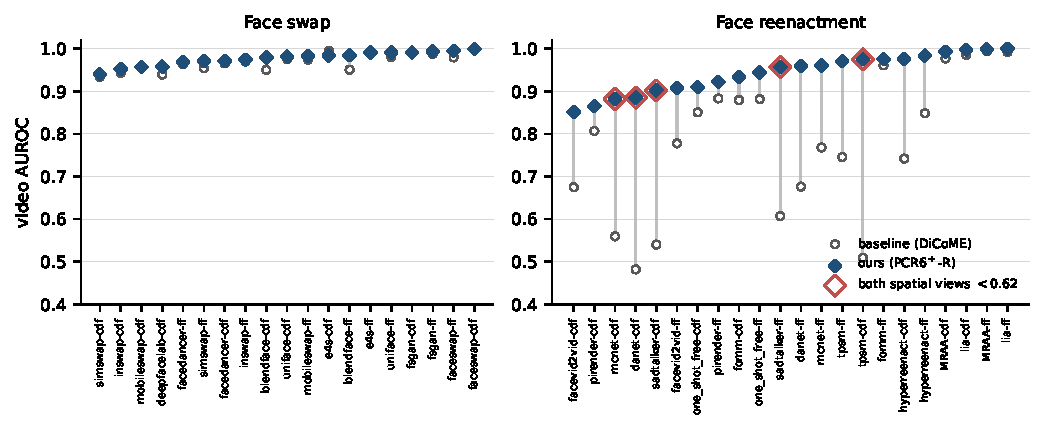
\includegraphics[width=\textwidth]{figures/fig_df40.pdf}
\caption{Per-generator video AUROC on all $41$ DF40 generator--source entries, sorted within each family by the
proposed system's score. Grey stems join the two systems on the same entry. Circled markers are the reenactment
generators on which both spatial views fall below $0.62$ AUROC. On face swapping the two systems are close and both
near the ceiling; on reenactment the baseline collapses on exactly the entries where per-frame evidence is absent.}
\label{fig:df40}
\end{figure*}

The per-entry table and Fig.~\ref{fig:df40} show why. On DaNet, MCNet, SadTalker and TPSM in the Celeb-DF-sourced set, both spatial views sit at or below $0.62$ AUROC -- at chance -- while the temporal view alone reaches $0.94$--$0.99$. These are precisely the generators that render individually plausible frames and betray themselves in motion, and they
are the shaded band of Fig.~\ref{fig:complementarity}. A two-view spatial system has nothing to combine on them, which is why the baseline falls to $0.48$--$0.55$ there. Because our spatial views are frozen at the baseline's own values, this gap is attributable to the temporal view and the fusion, not to a better spatial encoder.

We stress the symmetric observation: the system does not trade one family for the other. It is ahead on $17$ of $19$ swap entries as well, where the margin is small only because both systems are close to the ceiling.

\subsection{View necessity}
\label{sec:views}

% generated by analysis/tbiom/paper/build_tables.py
% source: EXP_PCR6P_DEVELOPMENT.json + EXP_PCR6P_EXPOSED.json
\begin{table}[t]
\centering
\caption{View subsets, each fitted and scored identically and fused with the proposed operator; only the view set changes. Best per column in \textbf{bold}. These are means taken across manipulation families and partly cancel the per-family effects; Table~\ref{tab:viewrole} resolves them.}
\label{tab:views}
\small
\begin{tabular}{lcccc}
\toprule
Views & Dev.\ v3.1 & Reenact. & 10-set & DF40 \\
\midrule
$T$ & 0.8094 & 0.9135 & 0.8213 & 0.9195 \\
$A{+}O$ & 0.8262 & 0.7644 & 0.8959 & 0.8804 \\
$T{+}A$ & 0.8693 & 0.9065 & 0.9003 & 0.9522 \\
$T{+}O$ & \textbf{0.8800} & \textbf{0.9157} & 0.9121 & \textbf{0.9624} \\
$T{+}A{+}O$ (deployed) & 0.8794 & 0.9111 & \textbf{0.9129} & 0.9602 \\
\bottomrule
\end{tabular}
\end{table}


\begin{figure}[t]
\centering
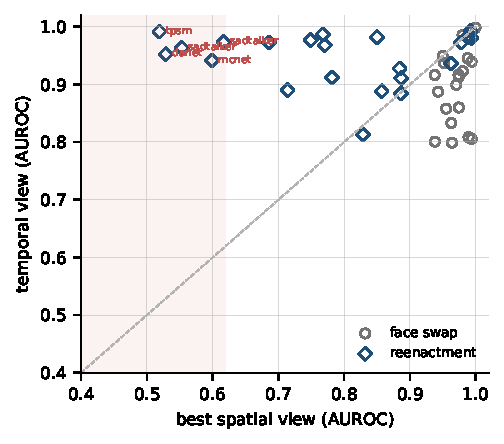
\includegraphics[width=\columnwidth]{figures/fig_complementarity.pdf}
\caption{Complementarity structure across the $41$ DF40 entries: the temporal view's AUROC against the better of the
two spatial views. Points above the diagonal are entries where motion evidence is the stronger signal. In the shaded
band both spatial views are near chance, and every point there is a reenactment generator.}
\label{fig:complementarity}
\end{figure}

Table~\ref{tab:views} fits and scores every view subset identically under the proposed operator, and
Table~\ref{tab:viewrole} reports what removing each view costs on each kind of evaluation content.

% generated by analysis/tbiom/paper/build_tables.py
% source: EXP_PCR6P_EXPOSED.json
\begin{table}[t]
\centering
\caption{What each view contributes, and where. Each column removes one view from the deployed set and reports the change in mean video AUROC. The views divide the work by manipulation family: the appearance view earns its place on swap and in-the-wild content, the off-manifold and temporal views on reenactment.}
\label{tab:viewrole}
\small
\begin{tabular}{lcccc}
\toprule
Evaluation group & Full & $-A$ & $-O$ & $-T$ \\
\midrule
Swap-dominated sets & 0.9267 & $-0.0015$ & $-0.0152$ & $+0.0097$ \\
Reenactment-heavy sets & 0.9620 & $+0.0027$ & $-0.0092$ & $-0.0941$ \\
In-the-wild sets & 0.8226 & $-0.0024$ & $-0.0083$ & $-0.0201$ \\
\midrule
DF40 face swap & 0.9770 & $-0.0010$ & $-0.0053$ & $-0.0080$ \\
DF40 reenactment & 0.9431 & $+0.0054$ & $-0.0110$ & $-0.1514$ \\
\bottomrule
\end{tabular}
\end{table}


\emph{The temporal view is necessary, and decisively so on reenactment.} Removing it costs $0.094$ on the
reenactment-heavy benchmarks and $0.151$ on the DF40 reenactment family -- an order of magnitude larger than any
other view's effect anywhere in the table. It also costs on in-the-wild content ($-0.020$) and on DF40 swaps
($-0.008$). The one place it does not help is the swap-dominated benchmarks ($+0.010$), where per-frame evidence is
abundant and motion adds little.

\emph{The off-manifold view is necessary everywhere.} It is the only view whose removal hurts every group, from
$-0.005$ on DF40 swaps to $-0.015$ on the swap-dominated benchmarks. It is the system's general-purpose spatial
evidence.

\emph{The appearance view is specialised rather than redundant.} Removing it costs on four of the five groups --
swap-dominated sets, in-the-wild sets, DF40 swaps -- and helps only on reenactment, where per-frame appearance is
by construction uninformative and an insistent spatial opinion is a liability. This is precisely the behaviour the
reliability discount is there to manage: the fitted weight is non-zero on the folds where appearance evidence is
useful and is driven to zero on those where it is not, so the view participates when it has something to say and
steps aside when it does not.

The aggregate ladder in Table~\ref{tab:views} should be read in that light. $T{+}O$ and the full system differ by
less than $0.003$ on any summary, because the appearance view's gains on swap content and its losses on reenactment
partly cancel in a mean taken across both. The family-resolved view in Table~\ref{tab:viewrole} is the informative
one, and it shows three views doing three different jobs.

\subsection{The fusion operator}

% generated by analysis/tbiom/paper/build_tables.py
% source: EXP_PCR6P_DEVELOPMENT.json, EXP_PCR6P_EXPOSED.json, EXP_PCR6P_AUDIT.json
\begin{table}[t]
\centering
\caption{Combination rules over the same three view opinions with the same fitted reliabilities. Only the operator changes. $\Delta_{r=0}$ is the largest change caused by removing a view the reliability fit has already discounted to zero: it is exactly zero only for the proposed rule.}
\label{tab:operators}
\small
\begin{tabular}{lcccc}
\toprule
Operator & Dev.\ v3.1 & 10-set & DF40 & $\Delta_{r=0}$ \\
\midrule
\textbf{PCR6$^+$-R (ours)} & 0.8794 & 0.9129 & 0.9602 & $0$ \\
PCR6-R & 0.8793 & 0.9134 & 0.9582 & $0.28$ \\
PCR6-R, pairwise fold & 0.8802 & 0.9147 & 0.9586 & -- \\
Yager-R & 0.8787 & 0.9124 & 0.9585 & -- \\
Averaging-R~\cite{rcml} & 0.8799 & 0.9141 & 0.9618 & -- \\
Dempster-R~\cite{shafer} & 0.8808 & 0.9155 & 0.9591 & -- \\
\bottomrule
\end{tabular}
\end{table}


Table~\ref{tab:operators} varies only the combination rule, holding the view opinions and the fitted reliabilities fixed. Detection differences among the rules are small: the spread across six operators is $0.0026$ on the ten-set mean. The rules are therefore not distinguished by accuracy, and we do not claim they are.

They are distinguished by the last column. Removing a view that the reliability fit has already discounted to zero changes the fused opinion by exactly $0$ under \pcrp{} and by up to $0.28$ under PCR6. Dempster's rule and the pairwise PCR6 fold share PCR6's defect. Since zero weights occur in most folds, this is the property that makes \pcrp{} the coherent choice for a reliability-discounted system, and it is why we adopt it despite a marginally lower mean AUROC than Dempster's rule.

Two labelling points are worth recording for reproducibility. PCR6 is not associative, so a sequential pairwise fold is a different operator from the direct multi-source rule; the two differ by up to $0.18$ on admissible opinions and are reported as separate rows. Yager's rule is likewise non-associative and is implemented directly.

\subsection{Reliability, calibration and robustness}
\label{sec:reliability}

% generated by analysis/tbiom/paper/build_tables.py
% source: EXP_PCR6P_EXPOSED.json
\begin{table}[t]
\centering
\caption{Calibration, selective prediction and processing robustness for the proposed system. Error-detection AUROC ranks the system's own mistakes; E-AURC is the excess area under the risk--coverage curve. JPEG and resize are applied at evaluation only; no arm was trained on them.}
\label{tab:reliability}
\small
\begin{tabular}{lccccc}
\toprule
Set & AUROC & ECE & NLL & err-AUROC & E-AURC \\
\midrule
CDF-v2 & 0.9583 & 0.254 & 0.516 & 0.641 & 0.1119 \\
CDF-v3 & 0.9639 & 0.283 & 0.517 & 0.768 & 0.0547 \\
DFD & 0.9307 & 0.220 & 0.456 & 0.790 & 0.0470 \\
FFIW & 0.9217 & 0.099 & 0.405 & 0.699 & 0.0749 \\
KoDF & 0.9600 & 0.128 & 0.345 & 0.821 & 0.0199 \\
IDForge & 0.9631 & 0.078 & 0.285 & 0.793 & 0.0314 \\
DFDM & 0.9954 & 0.060 & 0.108 & 0.897 & 0.0034 \\
\midrule
CDF-v2, JPEG q40 & 0.8683 & 0.482 & 1.311 & 0.646 & 0.2015 \\
CDF-v2, resize 0.6 & 0.9396 & 0.304 & 0.652 & 0.673 & 0.1258 \\
DFDCP, JPEG q40 & 0.8170 & 0.413 & 1.210 & 0.663 & 0.1635 \\
DFDCP, resize 0.6 & 0.8033 & 0.208 & 0.674 & 0.663 & 0.1366 \\
\bottomrule
\end{tabular}
\end{table}


Table~\ref{tab:reliability} reports calibration and selective prediction per benchmark, and the two evaluation-time corruptions. The fused vacuity is an informative error ranker, and risk falls monotonically as coverage is reduced, which is the behaviour a deployed system needs when it is allowed to abstain.

Under corruption the system degrades gracefully rather than collapsing: neither JPEG quality $40$ nor a $0.60$ down--up resize was seen in any fitting or selection step, and both are applied to the stored crops at evaluation only.

\section{Discussion and Limitations}

\textbf{What the evidence supports.} The strongest claim this paper makes is the controlled one: adding a temporal view to frozen spatial evidence changes reenactment detection substantially and swap detection marginally, in a direction and magnitude that the per-generator view scores explain. The weakest link in any contrary reading is the near-chance generators, where the spatial views are demonstrably uninformative and the temporal view is demonstrably not.

\textbf{What it does not support.} We do not claim a novel fusion operator: \pcrp{} is prior work and is credited
as such. We do not claim that the three views are jointly necessary on every kind of content -- Table~\ref{tab:viewrole}
shows the opposite, that each is dispensable somewhere and that the reliability fit exploits this. We do not claim
held-out generalisation from the DF40 or ten-set results, because both suites are exposed.

\textbf{Seeds and replication.} The five folds are fitting folds, not independent detector seeds. Results are reported for one deployed detector configuration; the spatial recipe exists at a single training seed and a second spatial seed would require retraining, which is outside this study's scope.

\textbf{Reliability as a fitted quantity.} Reliability weights are fitted once on development and held fixed at inference. Per-sample reliability estimation, as in~\cite{dbf}, is a natural extension and is not attempted here.

\section{Conclusion}
Face swapping and face reenactment place different demands on a detector, and the gap between them is not closed by a better spatial encoder. We showed that adding an adapted temporal view to frozen spatial evidence, and combining the three as subjective opinions under a reliability-aware conflict-redistribution rule, leaves swap performance essentially unchanged while changing reenactment performance substantially -- ahead on all $22$ reenactment entries of DF40 and on $39$ of $41$ overall. We also showed how the work divides: the temporal view carries reenactment, the off-manifold view contributes everywhere, the appearance view earns its place on swap and in-the-wild content, and the operator matters less for accuracy than for coherence with the reliability weights it is given.

\section*{Acknowledgment}
This material is based upon work supported by the National Science Foundation (NSF) under Grant number 2409577. Any
opinions, findings, and conclusions, or recommendations expressed in this material are those of the author(s) and do
not necessarily reflect the views of the NSF.

\bibliographystyle{IEEEtran}
\bibliography{refs}

\end{document}
